\documentclass[serif,mathserif,10pt]{beamer}
\usepackage{amsmath, amsfonts, epsfig, xspace}
\usepackage{algorithm,algorithmic}
\usepackage{pstricks,pst-node}
\usepackage{multimedia}
\usepackage[normal,tight,center]{subfigure}
\setlength{\subfigcapskip}{-.5em}
\usepackage{beamerthemesplit}
\usetheme{lankton-keynote}

\usepackage{mdframed}

\usepackage{setspace}% http://ctan.org/pkg/setspace
\let\oldframetitle\frametitle% Store \frametitle in \oldframetitle
\renewcommand{\frametitle}[1]{%
      \oldframetitle{#1}\setstretch{1.2}}

\hypersetup{colorlinks}

\newcommand{\matr}[1]{\mathbf{#1}}
\newcommand{\tran}[1]{#1^{\top}}

\def\gw#1{gravitational wave#1 (GW#1)\gdef\gw{GW}}
\def\ns#1{neutron star#1 (NS#1)\gdef\ns{NS}}
\def\prd{Phys. Rev. D.}
\def\apj{ApJ}

%\titlegraphic{
\includegraphics[width=0.5\textwidth]{figures/cra.png}}

\begin{document}
\setbeamertemplate{caption}{\raggedright\insertcaption\par}

\title[BNS Bursts]{Searching For Gravitational Wave Bursts From
Binary Neutron Star Coalescence}
\author{James A. Clark}
\institute{Georgia Institute of Technology}
\date{} 

%\maketitle

\begin{frame}[plain]
\titlepage
\small{With contributions from and thanks to: A.~Bauswein, A.~Maselli,
C.~Lazzarro, B.~Giacomazzo, N.~Stergioulas, W.~Kastaun, G.~Prodi, R.~Ciolfi,
M.~Coughlin, S.~Coughlin, M.~Tringali\dots}
\end{frame}

\begin{frame}
    \frametitle{This Talk}
    \centering
    \tableofcontents
\end{frame} 

\section{Motivation}

\subsection{GW Bursts From BNS Mergers}

\begin{frame}
    \frametitle{Burst Signals: Short}

    \begin{columns}

        \column{0.6\textwidth}

        {\small 
        \begin{itemize}
            \item BNS mergers: likely formation of a stable / quasi-stable,
                differentially rotating neutron star
                remnant~\cite{shibata:06bns, giacomazzo:11, hotokezaka:11,
                bauswein:12}.
            \item Transient non-axisymmetric deformations and $f$-mode oscillations
                $\rightarrow$ short (10--100\,ms) burst of high-frequency ($\sim $\,kHz)
                \gw{} emission.
            \item Spectral properties $\rightarrow$ neutron star equation of
                state from (e.g.,) dominant peak frequency $f_{\rm
                peak}$~\cite{hotokezaka:13,bauswein:14}.
            \item May be observable to $\sim$10's\,Mpc in advanced LIGO (c.
                2020+).
        \end{itemize}
    }

        \column{0.4\textwidth}

        \begin{center}
            \vspace{-0.1cm}
            \begin{figure}
                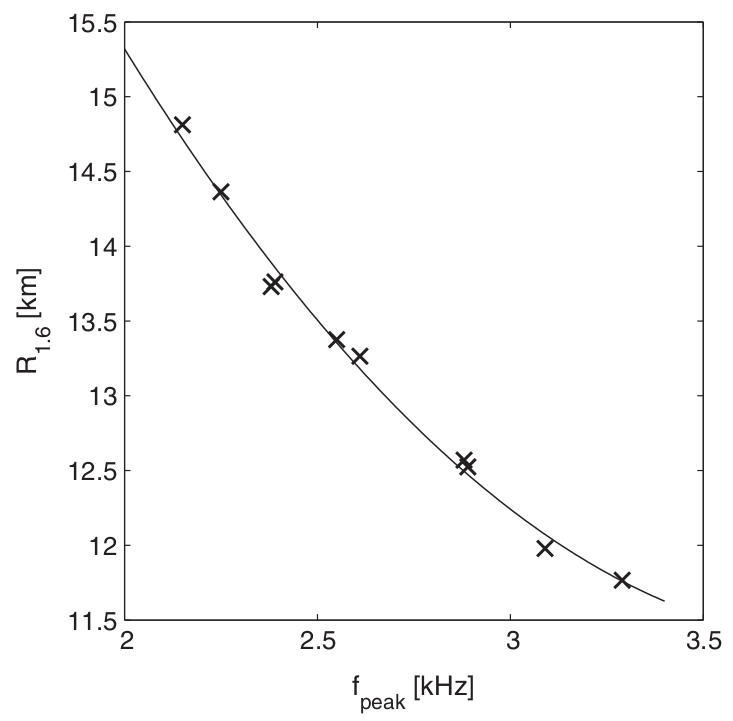
\includegraphics[width=1\columnwidth]{figures/fpeakR16.png}
                \caption{Peak-frequency/fiducial-radius relation
                from~\cite{bauswein:14}}
            \end{figure}
        \end{center}

    \end{columns}

\end{frame}

\begin{frame}
    \frametitle{BNS Burst Signals: Merger/Post-Merger}
    \begin{figure}
        \centering
        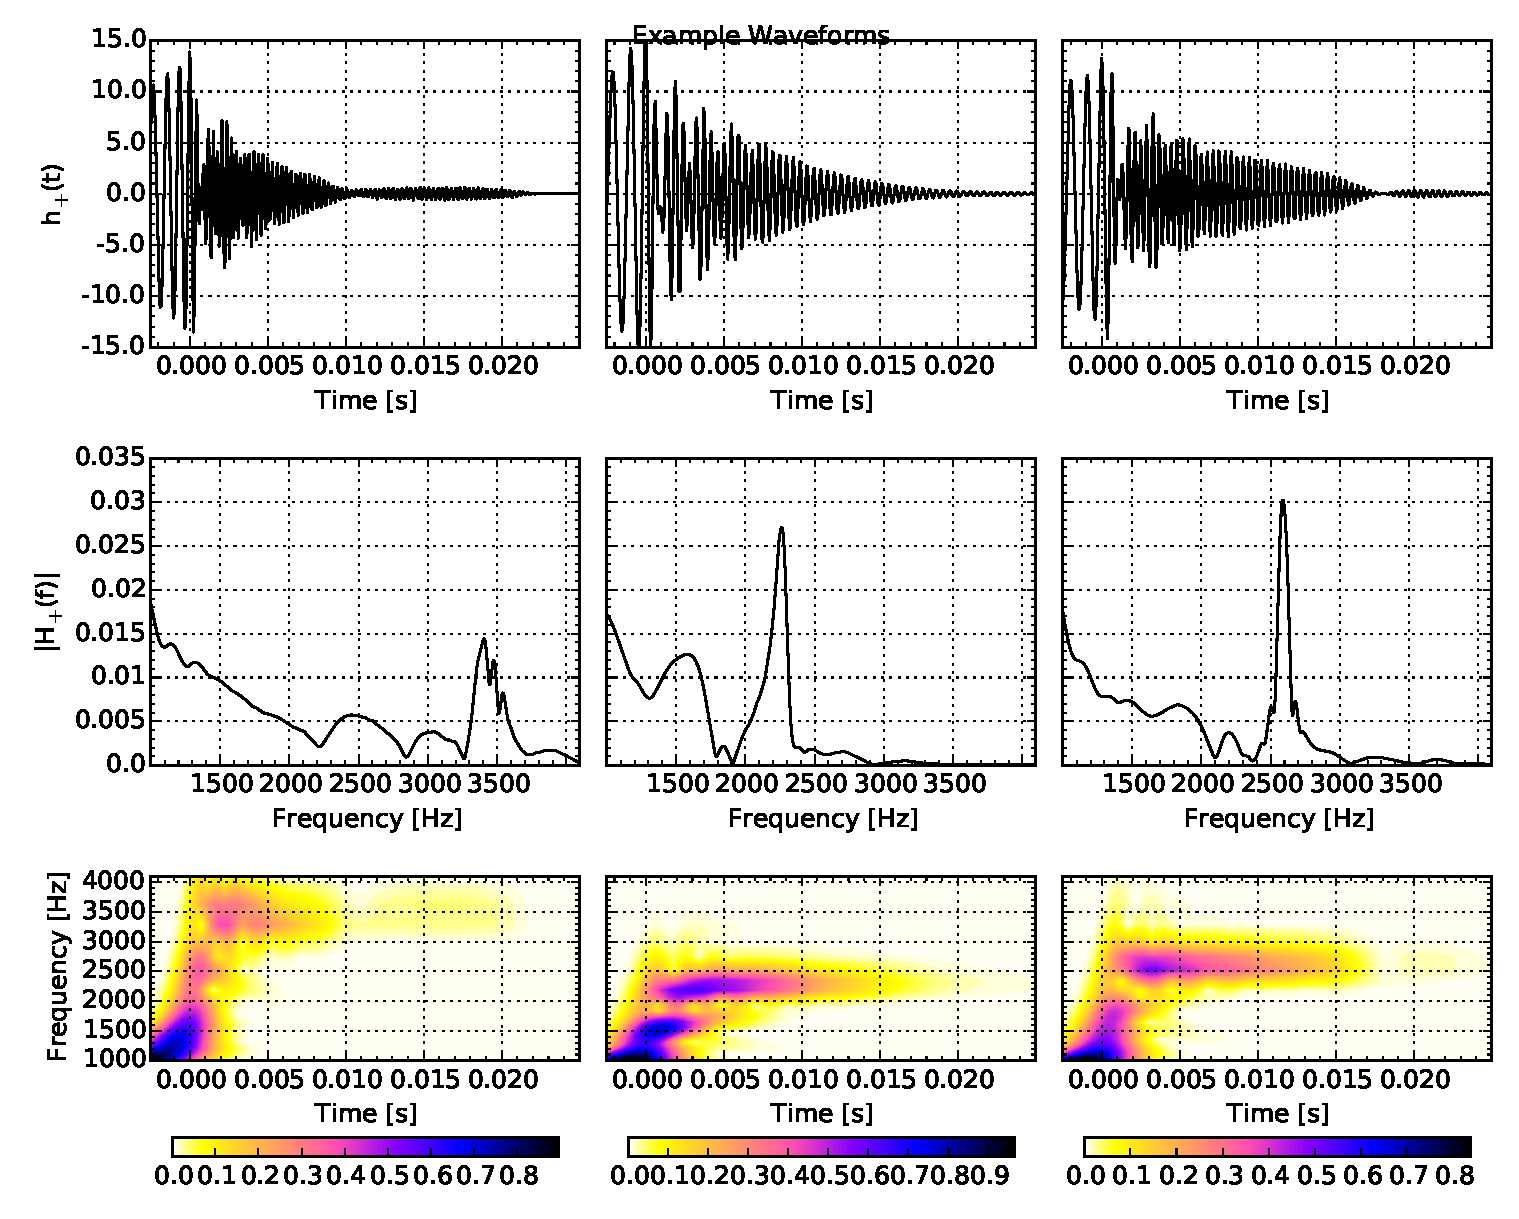
\includegraphics[width=0.75\columnwidth]{figures/example_waves.pdf}
        \caption{Examples for different EOS (APR, Shen, DD2).  Waveforms taken
        from~\cite{2014PhRvD..90f2004C}.}
    \end{figure}
\end{frame}

\section{Past/Present Analyses}

\subsection{GW Burst Analysis \& BNS Bursts}

\begin{frame}
    \frametitle{GW Burst Search: Coherent WaveBurst (CWB)}
    \begin{itemize}
        \item Search for excess power in time-frequency plane
        \item Decompose data with multi-resolution wavelet basis
        \item Coherent analysis maximises likelihood over waveform \&
            sky-location~\cite{Klimenko:2005wa,Klimenko:2007hd}
        \item Identifies statistically significant coherent power (detection),
            reconstructs GW signal
    \end{itemize}

    \begin{columns}

        \column{0.6\textwidth}

        \begin{center}
            \vspace{-0.1cm}
            \begin{figure}
                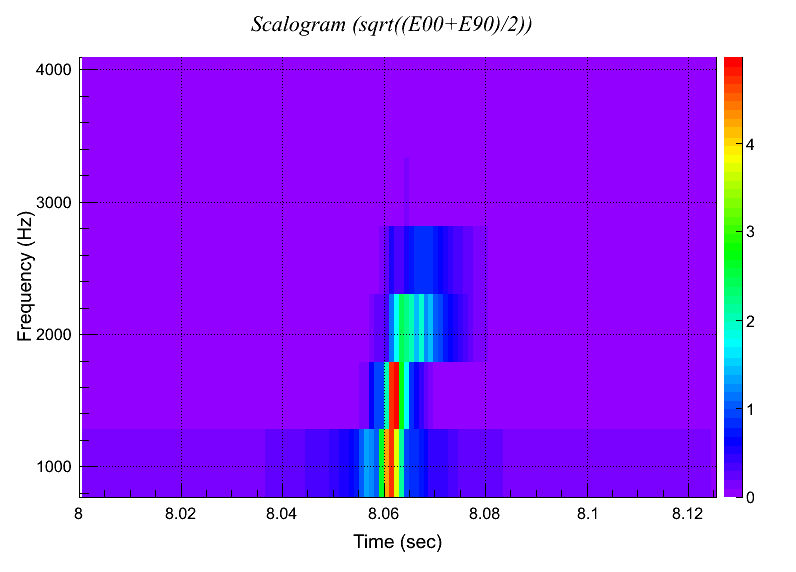
\includegraphics[width=0.7\columnwidth]{figures/L1_wf_white_inj_tf.png}
                \caption{Simulated signal}
            \end{figure}
        \end{center}

        \column{0.6\textwidth}

        \begin{center}
            \vspace{-0.1cm}
            \begin{figure}
                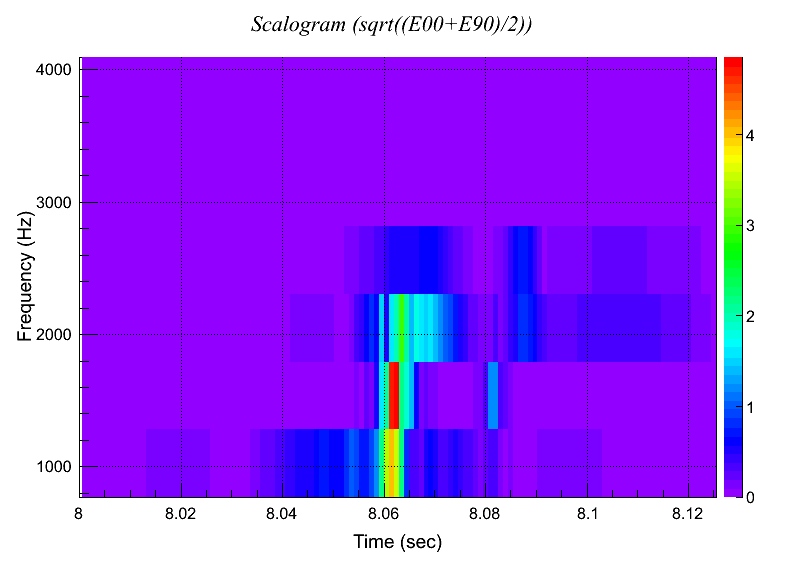
\includegraphics[width=0.7\columnwidth]{figures/L1_wf_white_rec_tf.png}
                \caption{Reconstructed signal}
            \end{figure}
        \end{center}

    \end{columns}

\end{frame}

\begin{frame}
    \frametitle{Previous Burst Detectability Study}
    \begin{quote}
        "Prospects For High Frequency Burst Searches Following Binary Neutron
        Star Coalescence With Advanced Gravitational Wave
        Detectors"~\cite{2014PhRvD..90f2004C}
    \end{quote}

    Monte-Carlo analysis of burst detectability and basic parameter estimation
    of post-merger bursts
    \begin{itemize}
        \item Family of numerical waveforms with various EoS
        \item Initial detector era noise recoloured to ~2022 sensitivities
        \item Deployed CWB to detect \& reconstruct signals
        \item Compared sensitivity with optimal matched filter expectation
        \item Very simple model selection procedure for spectral analysis of
            reconstructed signals (identify post-merger scenario, measure
            dominant frequency)
    \end{itemize}

\end{frame}


\begin{frame}
    \frametitle{Detectability \& Frequency Recovery}

    \begin{columns}[]

        \column{0.5\textwidth}

        \begin{center}
            \vspace{-0.08cm}
            \begin{figure}
                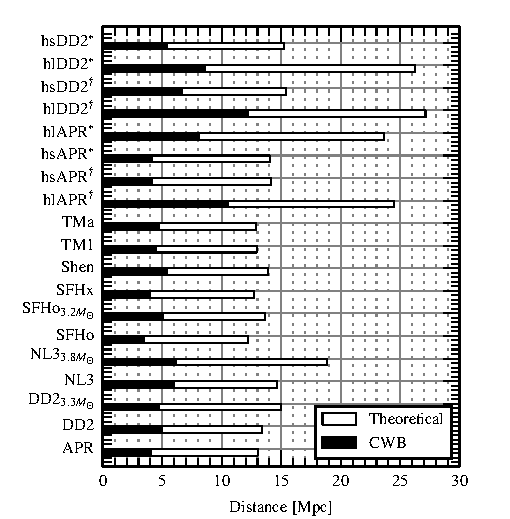
\includegraphics[width=1\columnwidth]{figures/distances.pdf}
                \caption{Effective range for theoretical matched
                    filter \& burst analysis (fixed false alarm
                    probability=1\%)}
            \end{figure}
        \end{center}

        \column{0.5\textwidth}

        \begin{center}
            \vspace{-0.5cm}
            \begin{figure}
                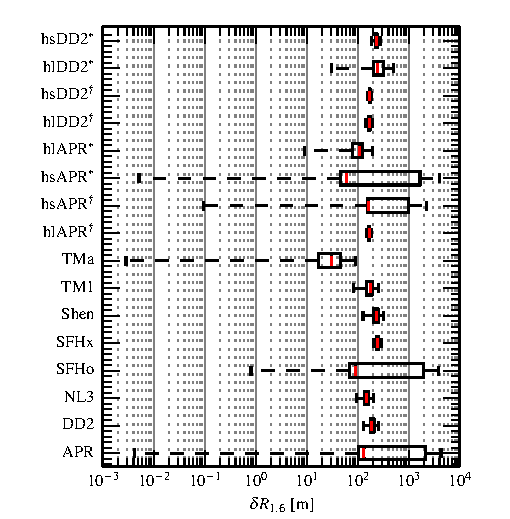
\includegraphics[width=1\columnwidth]{figures/deltaRadii.pdf}
                \caption{Absolute error in radius recovery, using $f_{\rm
                peak}-R_{1.6}$ relation in~\cite{bauswein:12}.}
            \end{figure}
        \end{center}

    \end{columns}

\end{frame}



\begin{frame}
    \frametitle{New Study: Prospects for\dots: Round 2}
    Motivation \& Goals of Study:
    \begin{itemize}
        \item Recent upgrades to flagship burst analysis algorithm \footnote{e.g.,
            multi-resolution analysis}
        \item More post-merger waveforms from University of Trento (also
            home of various CWB experts)
        \item Point-comparison of SPH and NR waveform codes from independent
            groups
        \item Also recent development \& availability of `unmodelled' Bayesian
            analysis algorithm
        \item Tune the post-merger analysis for next year's BNS inspiral detection!
    \end{itemize}

    Participants from GATech, Universities of Thessaloniki \& Trento

\end{frame}


%\begin{frame}
%    \frametitle{Preliminary Results From New Study}
%    New analysis just beginning but some interesting studies already
%    \begin{itemize}
%        \item Going further than previous study and looking at
%            full-reconstruction fidelity characterised by match \emph{and}
%            peak frequency measurements
%        %\item Still probing sensitivity \& optimising thresholds
%    \end{itemize}
%
%
%    \begin{columns}
%
%        \column{0.5\textwidth}
%
%        \begin{center}
%            \vspace{-0.1cm}
%            \begin{figure}
%                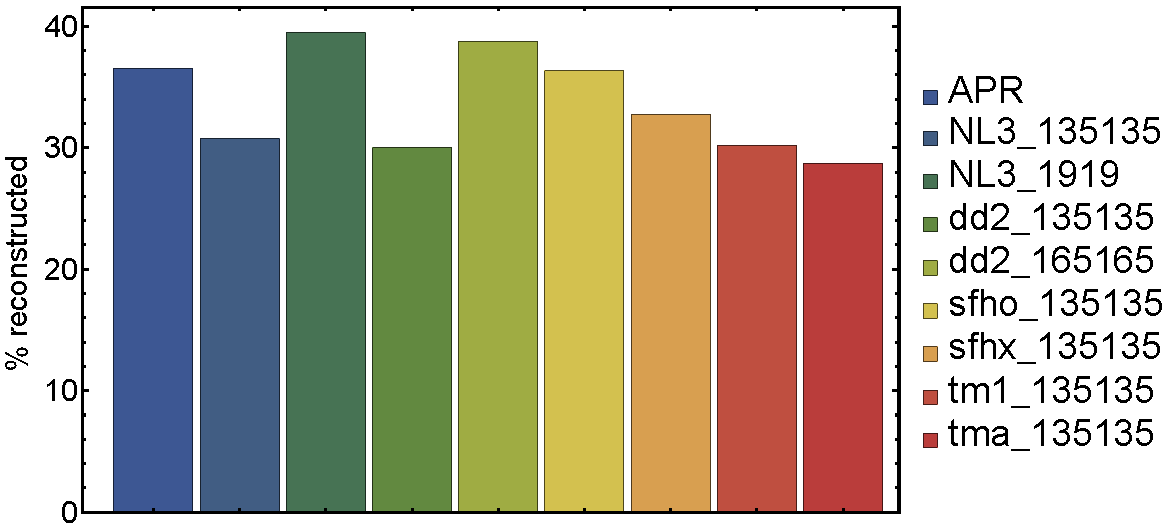
\includegraphics[width=1.0\columnwidth]{figures/thess_events.pdf}
%                \caption{Fraction of signals detected at 4\,Mpc}
%            \end{figure}
%        \end{center}
%
%        \column{0.5\textwidth}
%
%        \begin{center}
%            \vspace{-0.1cm}
%            \begin{figure}
%                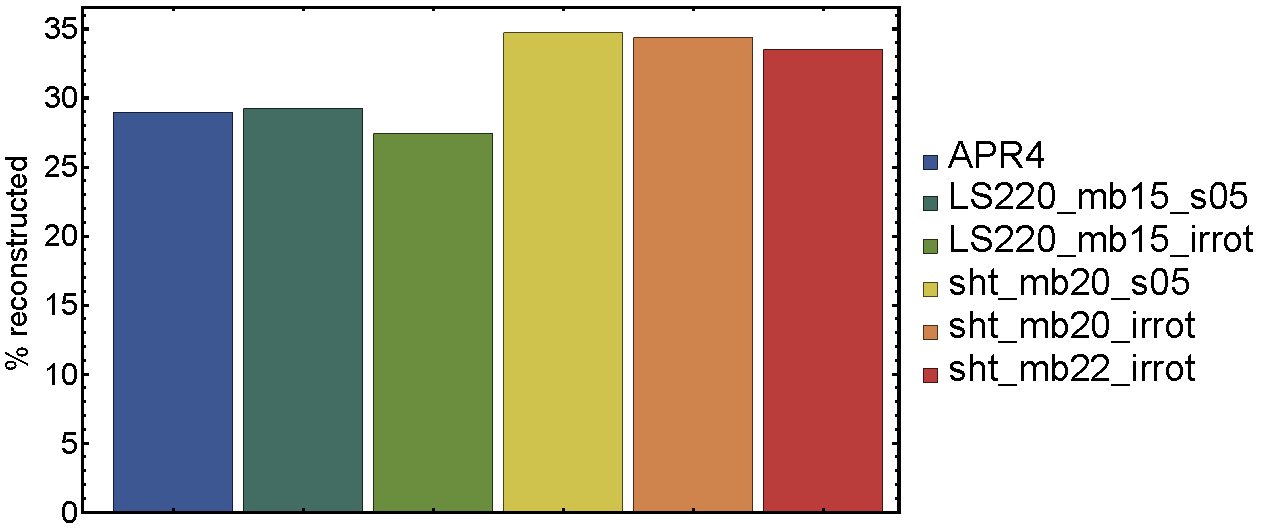
\includegraphics[width=1.0\columnwidth]{figures/trento_events.pdf}
%                %\caption{Reconstructed signal}
%            \end{figure}
%        \end{center}
%
%    \end{columns}
%
%\end{frame}


\begin{frame}
    \frametitle{Preliminary Results From New Study}
    \begin{itemize}
        \item Going further than previous study and looking at
            full-reconstruction fidelity characterised by match \emph{and}
            peak frequency measurements
        %\item Still probing sensitivity \& optimising thresholds
        \item `Ceiling' on matches $\rightarrow$ Missing
            late-time/high-frequency post-merger signal; goal is to tune the
            analysis to avoid this effect
    \end{itemize}


    \begin{columns}

        \column{0.5\textwidth}

        \begin{center}
            \vspace{-0.1cm}
            \begin{figure}
                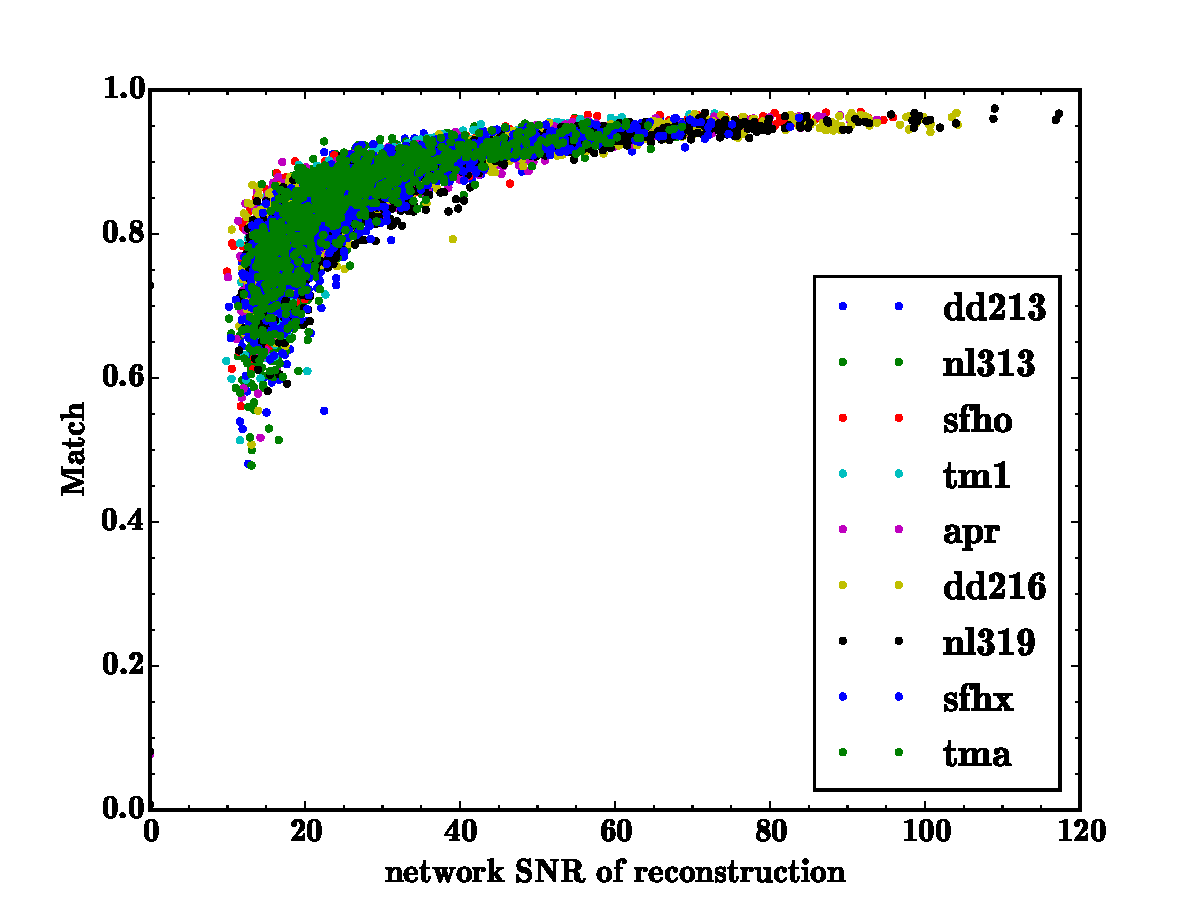
\includegraphics[width=1.0\columnwidth]{figures/recSNR_vs_match.pdf}
                %\caption{Reconstruction Fidelity (match=noise-weighted inner
                %product)}
            \end{figure}
        \end{center}

        \column{0.5\textwidth}

        \begin{center}
            \vspace{-0.1cm}
            \begin{figure}
                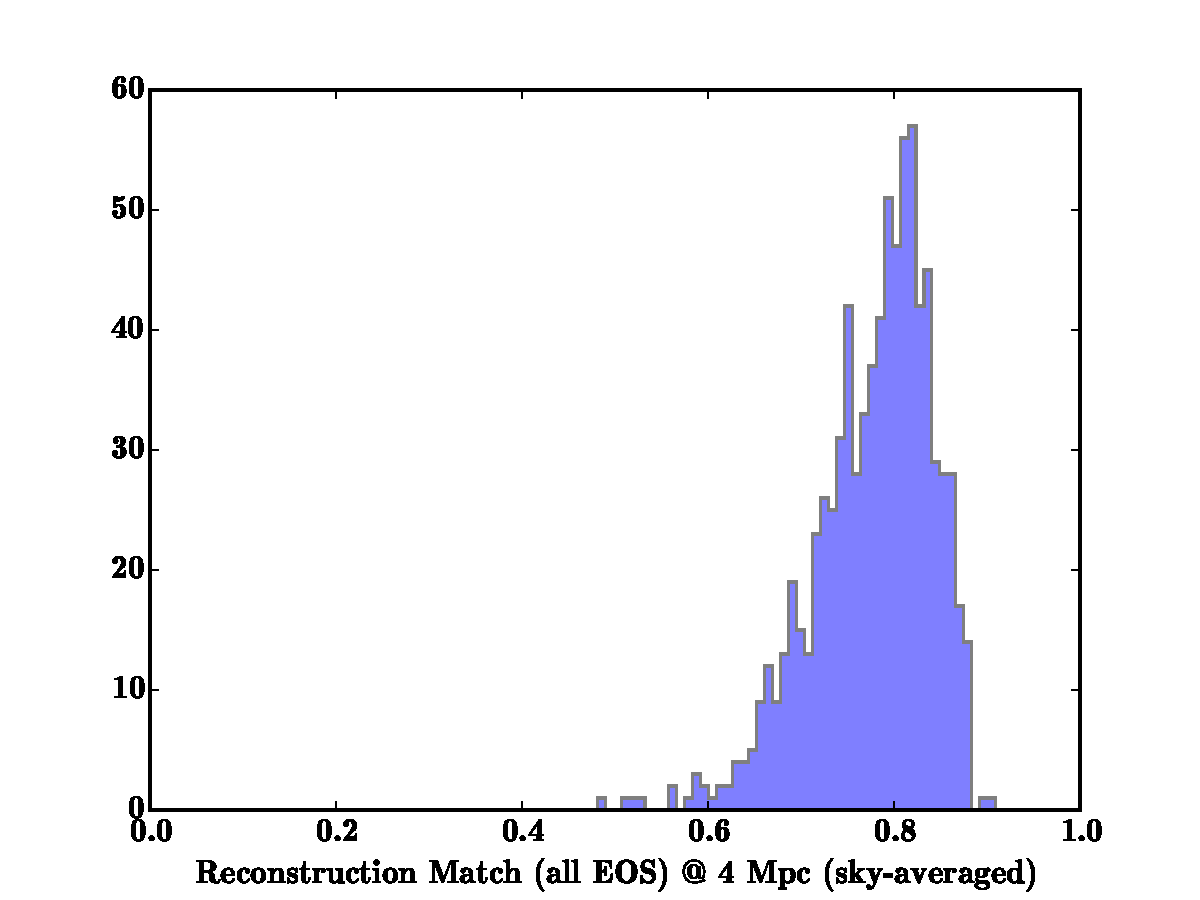
\includegraphics[width=1.0\columnwidth]{figures/small_scale_matches.pdf}
                %\caption{Reconstructed signal}
            \end{figure}
        \end{center}

    \end{columns}

\end{frame}

\section{Future Directions \& Developments}

\subsection{New Data Analysis Techniques}

\begin{frame}
    \frametitle{Enhancements \& Bayesian Methods}
    \begin{itemize}
        \item CWB: fast, robust \& familiar `flagship' burst analysis; principal
            tool GW burst searches.
        \item Other recent efforts for burst waveform recovery \&
            characterisation:
    \end{itemize}
        \begin{enumerate}
            \item Bayesian wavelet analysis (`BayesWave'); model dimension
                estimation \& potential to encode prior information on
                time-frequency structure
           \item Principal component analysis as a route to phenomelogical
               templates 
       \end{enumerate}
\end{frame}

\begin{frame}
    \frametitle{Principal Component Analysis Of Short Bursts}
    Clark, Bauswein \& Stergioulas (\emph{in prep.})
    \begin{small}
    \begin{enumerate}
        \item Goal: find a robust basis to accurately represent simulated
            waveforms
        \item Organise $M$ simulation waveforms, each containing $N$ samples,
            from numerical simulations of binary neutron star mergers into an
            $M\times N$ data matrix, $\matr{X}$
        \item Align dominant features, subtract the
            mean waveform $\bar{h}$ to get centered data matrix $\matr{Y}$
        \item Eigenvectors $\matr{W}$ of the covariance matrix
            $\matr{C} \sim \matr{Y}\tran{\matr{Y}}$ provide a basis to represent
            deviations from the mean
        \item Arbitrary waveform $h$ is represented in the new basis by,
            \begin{equation}
                h = \bar{h} + \sum_{i=1}^p \beta_i w_i,
            \end{equation}
            where $w_i$ are rows of $\matr{W}$ \& $\beta_i$ are projection
            coefficients from $\matr{B}=h'.\matr{W}$ 
        \item See e.g., supernova waveform analyses~\cite{2012PhRvD..86d4023L},
            reduced order modelling for BBH~\cite{2014CQGra..31s5010P}
    \end{enumerate}
\end{small}
\end{frame}


\begin{frame}
    \frametitle{Short Burst PCA}
    Clark, Bauswein \& Stergioulas (\emph{in prep.})

    \begin{figure}
        \centering
        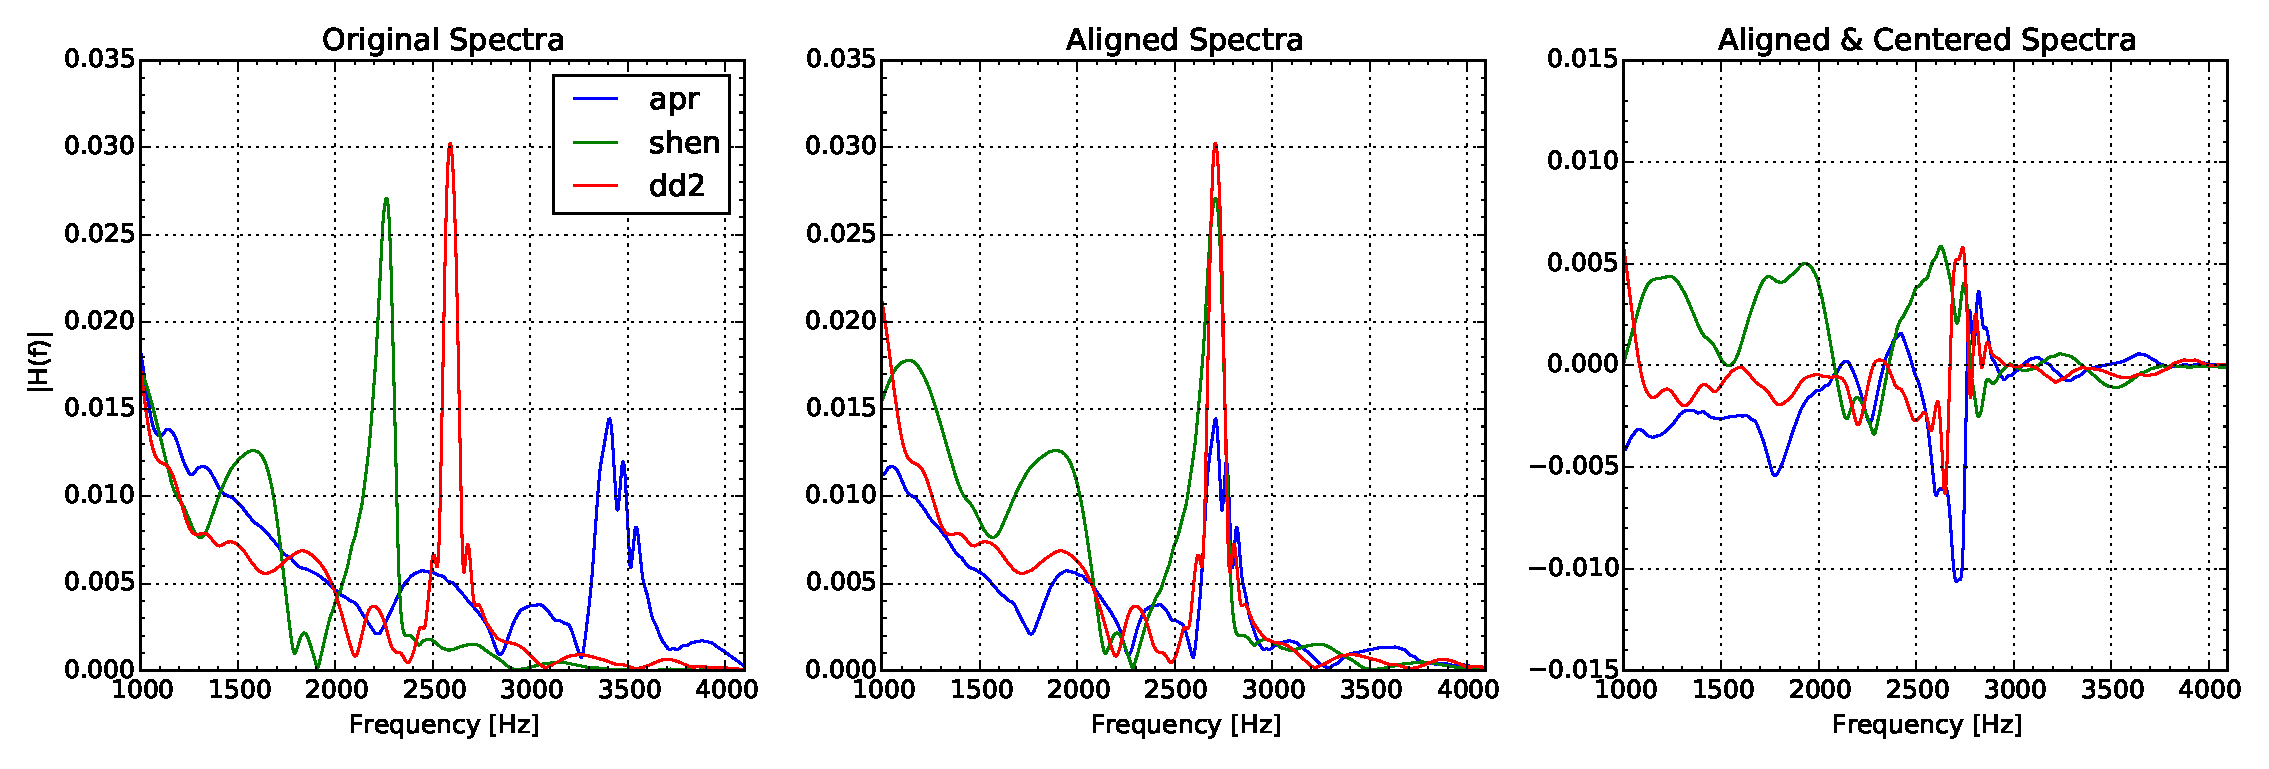
\includegraphics[width=\columnwidth]{figures/spectrum_conditioning_demo.pdf}
    \end{figure}

    \begin{figure}
        \centering
        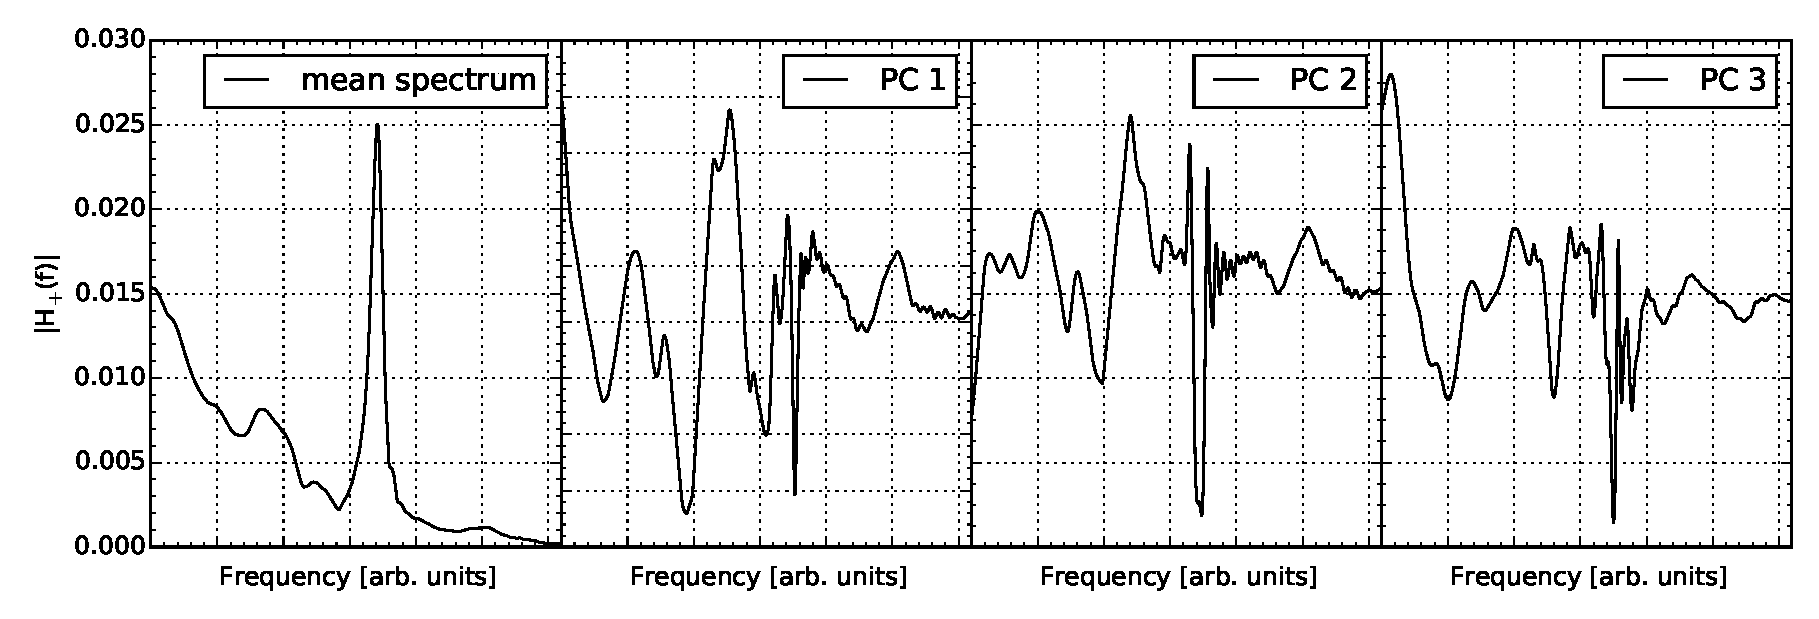
\includegraphics[width=\columnwidth]{figures/magnitude_pcs.pdf}
    \end{figure}

\end{frame}

\begin{frame}
    \frametitle{Prospects for PCA Of Short Bursts}

    \begin{columns}[]

        \column{0.5\textwidth}

%       \begin{center}
%           \vspace{-0.5cm}
%           \begin{figure}
%               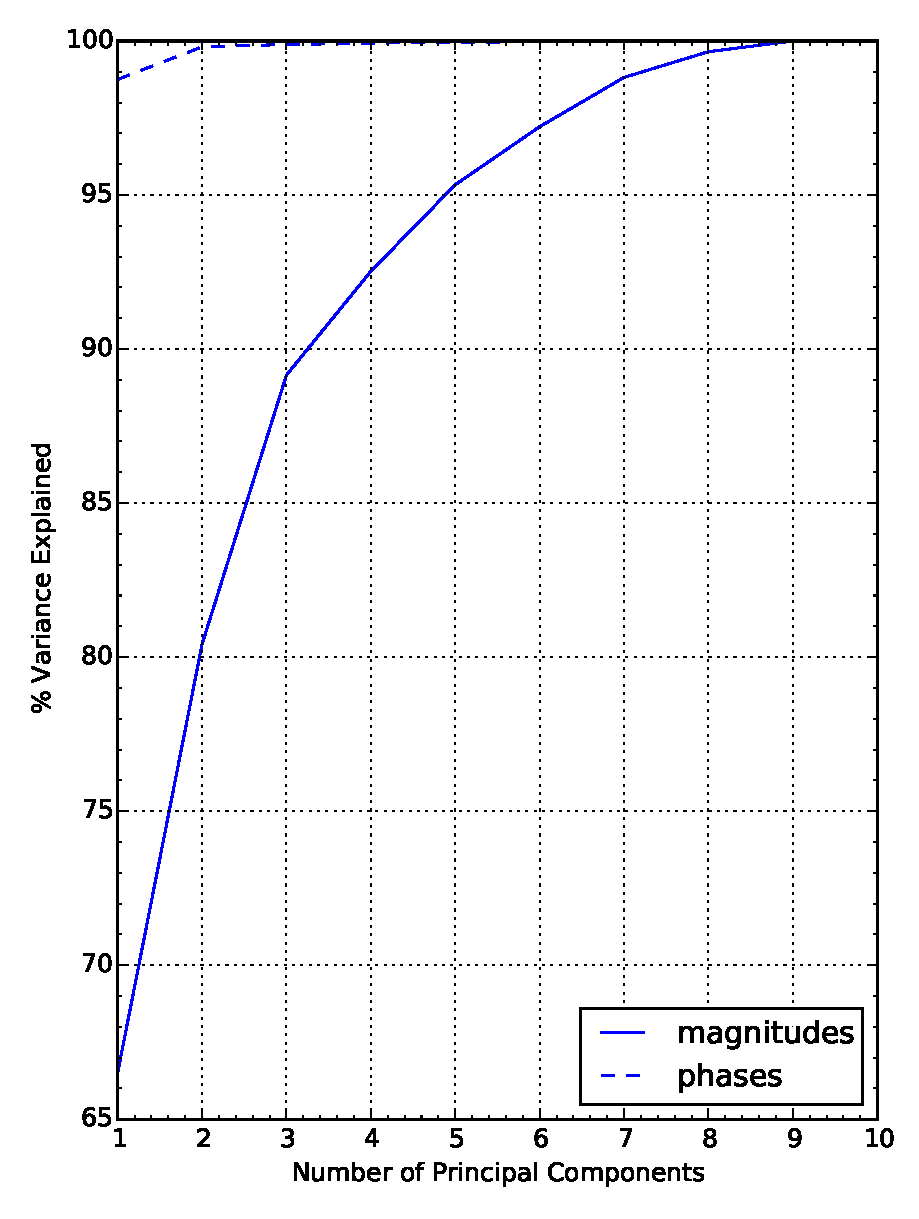
\includegraphics[width=\columnwidth]{figures/explained_variance.pdf}
%           \end{figure}
%       \end{center}


        PCA provides an (approximate) template:
        \begin{equation}
            H(f) \approx A_{\rm PCA}(f) \exp [i \phi_{\rm PCA}(f)],\nonumber
        \end{equation}
        where,
        \begin{eqnarray}
            A_{\rm PCA}(f) = \sum_{i=1}^N \beta_i^{(A)}u_i^{(A)} \\ \nonumber
            \phi_{\rm PCA}(f) = \sum_{i=1}^N \beta_i^{(\phi)}u_i^{(\phi)} \nonumber
        \end{eqnarray}

        Right: matches for waveforms in~\cite{2014PhRvD..90f2004C} using 1st
        principal component ($N=1$) from training data with test waveform
        excluded

        \column{0.5\textwidth}

        \begin{center}
            \vspace{-0.5cm}
            \begin{figure}
                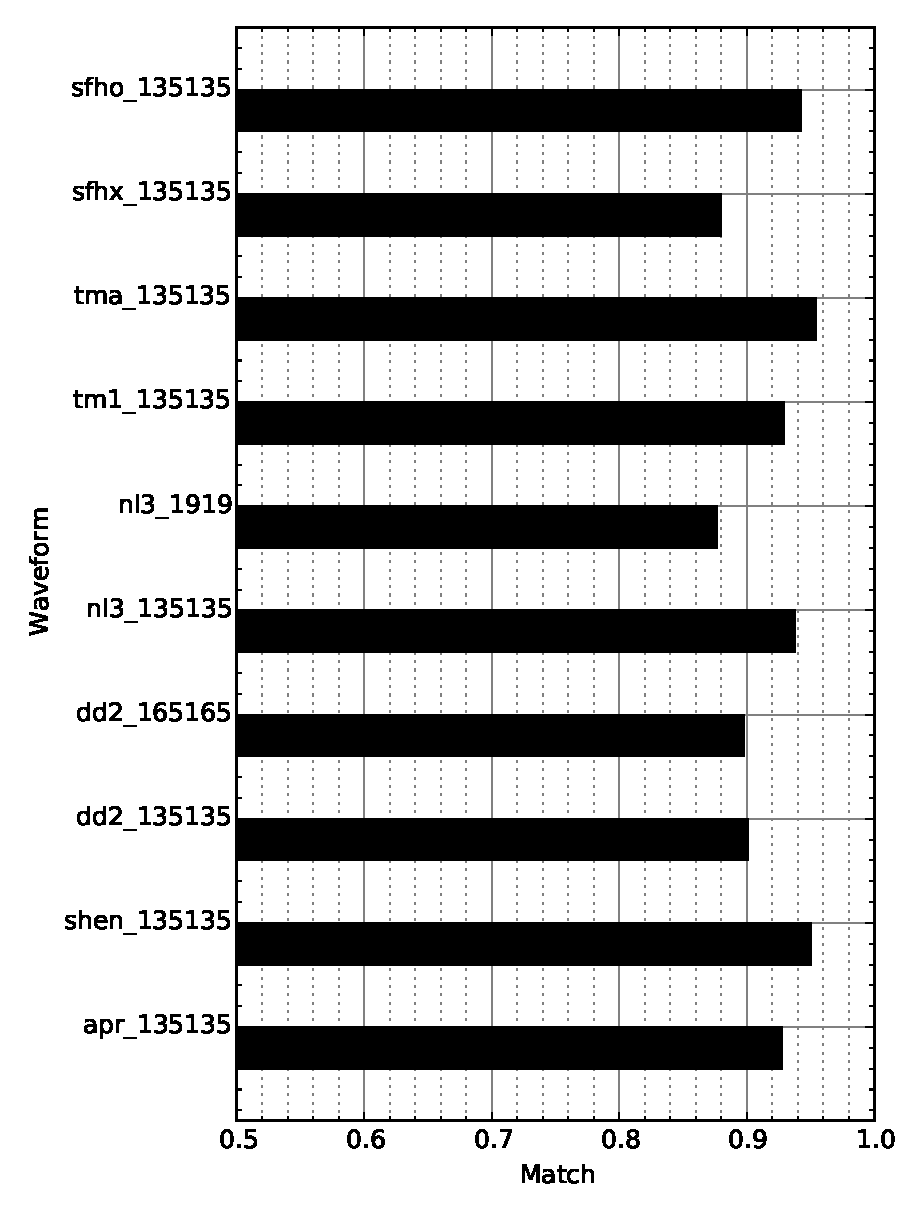
\includegraphics[width=\columnwidth]{figures/match_bars_exctestwav.pdf}
            \end{figure}
        \end{center}


    \end{columns}

\end{frame}

%\begin{frame}
%    \frametitle{Next Steps With PCA}
%
%    PCA provides an (approximate) template:
%    \begin{equation}
%        H(f) \approx A_{\rm PCA}(f) \exp [i \phi_{\rm PCA}(f)],
%    \end{equation}
%    where,
%    \begin{eqnarray}
%        A_{\rm PCA}(f) = \sum_{i=1}^N \beta_i^{(A)}u_i^{(A)} \\ \nonumber
%        \phi_{\rm PCA}(f) = \sum_{i=1}^N \beta_i^{(\phi)}u_i^{(\phi)} 
%    \end{eqnarray}
%
%    \begin{itemize}
%        \item Intrinsic parameters: peak frequency (used for feature alignment)
%            \& projection coefficients $\{\beta^{(A)}, \beta^{(\phi)}\}$
%        \item Yield approximate waveform reconstruction \\
%        \item Recover dominant \& sub-dominant frequencies \\
%    \end{itemize}
%
%    Implementation in LSC Bayesian inference packages coming soon \dots
%
%\end{frame}

\subsection{Long-duration Signals}

\begin{frame}
    \frametitle{Burst Signals: Long}

    Longer, louder GW emission also possible with formation of stable
    post-merger remnants.  Examples include:

    \begin{columns}


        \column{0.5\textwidth}

        \begin{center}
            \vspace{-0.1cm}
            \begin{figure}
                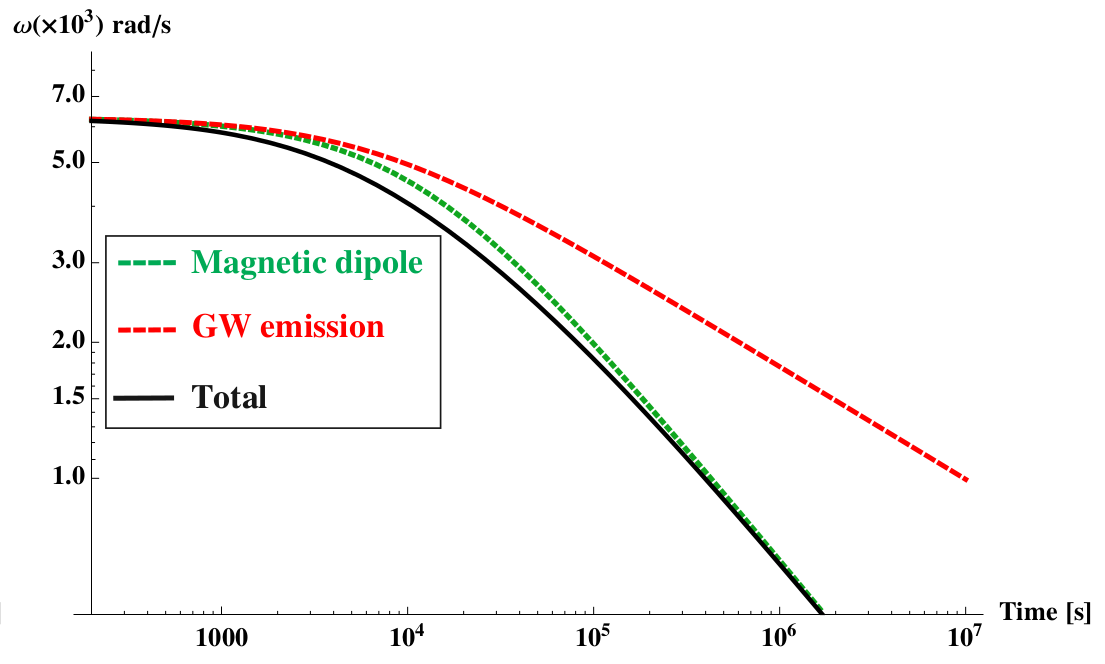
\includegraphics[width=1\columnwidth]{figures/dallosso.png}
                \caption{Magnetic field amplification $\rightarrow$ stable
                magnetar with $B$-field induced quadrupole
            moment~\cite{2015ApJ...798...25D}.  Emission over $\sim 10^6$\,s,
        matched-filter effective range: $\sim 25-53$\,Mpc}
            \end{figure}
        \end{center}

        \column{0.5\textwidth}

        \begin{center}
            \vspace{-0.1cm}
            \begin{figure}
                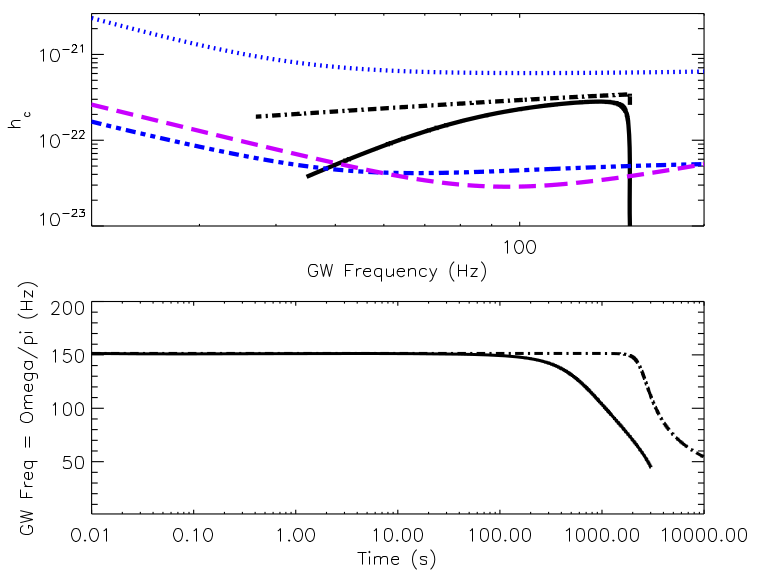
\includegraphics[width=1\columnwidth]{figures/corsi.png}
                \caption{Secular bar-mode instability~\cite{corsi:09}.
                Emission over $\sim$few$\times 10^2-10^3$\,s, matched-filter
            effective range: $\sim 45$\,Mpc.}
            \end{figure}
        \end{center}

    \end{columns}


\end{frame}


\begin{frame}
    \frametitle{Searching For Long Bursts}
%   Burst analyses typically tuned, focussed on ${\mathcal O}($s)-duration
%   transients. \\~\\
%
    Also have tools to specifically target long (few 100--few 1000s)
    transients, where precise morphology is unknown.  E.g., `STAMP'
    analysis~\cite{2011PhRvD..83h3004T}:

    \begin{columns}

        \column{0.5\textwidth}
        \begin{itemize}
            \item Cross-correlate strain time series from pairs of detectors
            \item Form cross-power time-frequency maps (e.g., right)
            \item Pattern-recognition problem: search for `tracks' in
                cross-power maps
        \end{itemize}

        \column{0.5\textwidth}
        \begin{center}
            \vspace{-0.1cm}
            \begin{figure}
                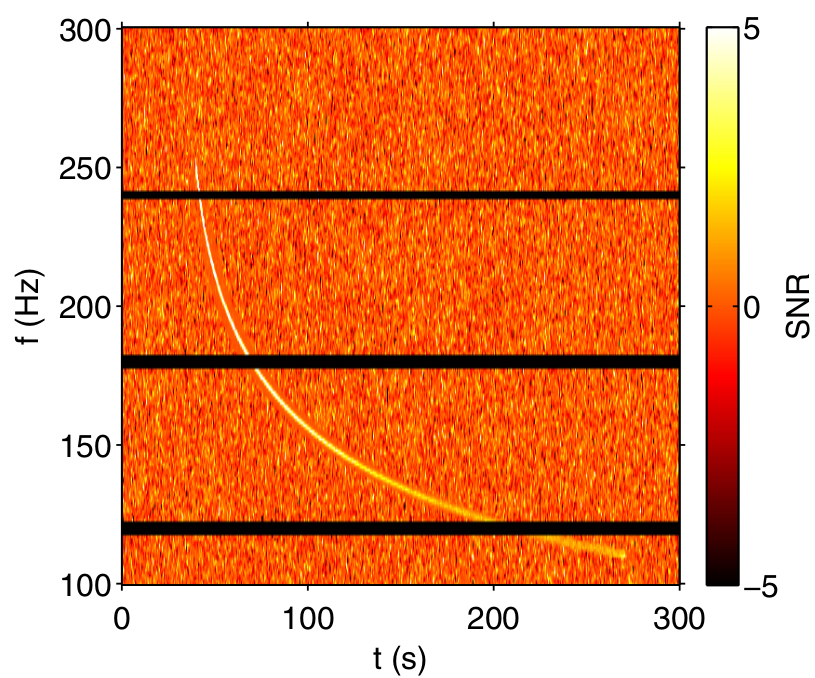
\includegraphics[width=0.8\columnwidth]{figures/stampadi.png}
                \caption{Example signal recovery with STAMP (accretion disk
                instability waveform).}  %Black regions: notched frequencies to
            %avoid instrumental lines.}
            \end{figure}
        \end{center}

    \end{columns}

    Sensitivity studies \& tuning now underway; interested in any/all
    long-transient signal scenarios

\end{frame}

\subsection{Summary \& Outlook}
\begin{frame}
    \frametitle{Summary}
    \begin{itemize}
        \item Likely formation of post-merger NS remnant following coalescence
        \item GWs from merger \& oscillations could constrain EOS for nearby
            mergers
        \item Challenges: weak signal \& uncertain morphology; use unmodelled
            burst analysis
        \item Initial burst study: signals observable in advanced detectors to a few
            Mpc, dominant post-merger frequencies quite well recovered.
        \item Follow-up burst study underway: multi-resolution analysis,
            opportunity to tune, study more waveforms \& characterise full
            waveform reconstruction fidelity
        \item Exciting new developments: PCA-based analysis could triple our
            range \& mature long-duration transient searches ready to go
    \end{itemize}
\end{frame}

\begin{frame}[allowframebreaks]
    \frametitle{References}
    \bibliographystyle{unsrt}
    \tiny{
        \bibliography{bns_bursts_clark}
}
\end{frame}

\appendix

\section{Detailed Results}

\begin{frame}
    \frametitle{Detectability \& Frequency Recovery}

    \begin{columns}[]

        \column{0.5\textwidth}

        \begin{center}
            \vspace{-0.08cm}
            \begin{figure}
                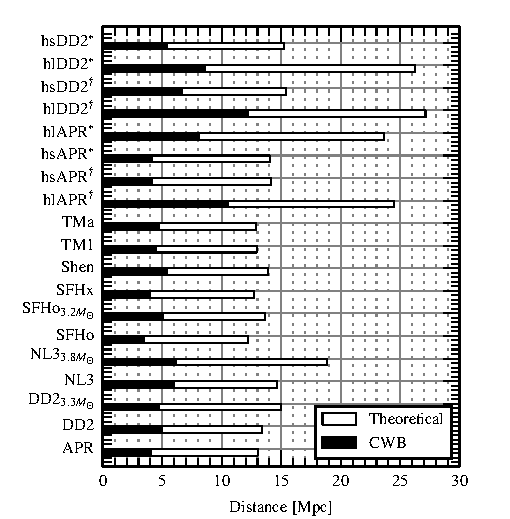
\includegraphics[width=1\columnwidth]{figures/distances.pdf}
                \caption{Effective range for theoretical matched
                    filter \& burst analysis (fixed false alarm
                    probability=1\%)}
            \end{figure}
        \end{center}

        \column{0.5\textwidth}

        \begin{center}
            \vspace{-0.5cm}
            \begin{figure}
                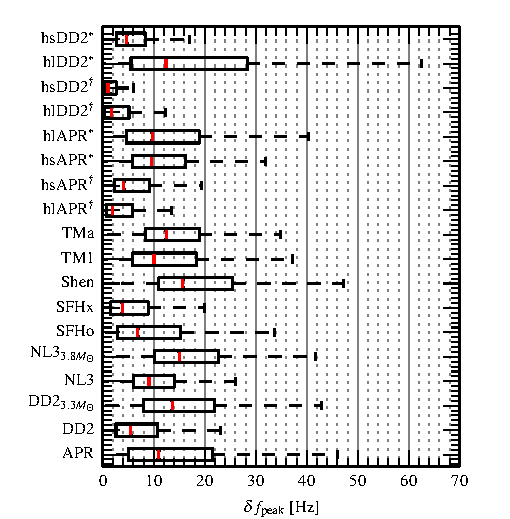
\includegraphics[width=1\columnwidth]{figures/deltaFpeak.pdf}
                \caption{Absolute error in peak frequency recovery}
            \end{figure}
        \end{center}

    \end{columns}

\end{frame}

\begin{frame}
    \frametitle{Classification Accuracy \& Radius Recovery}

    \begin{columns}[]

        \column{0.5\textwidth}

        \begin{center}
            \vspace{-0.08cm}
            \begin{figure}
                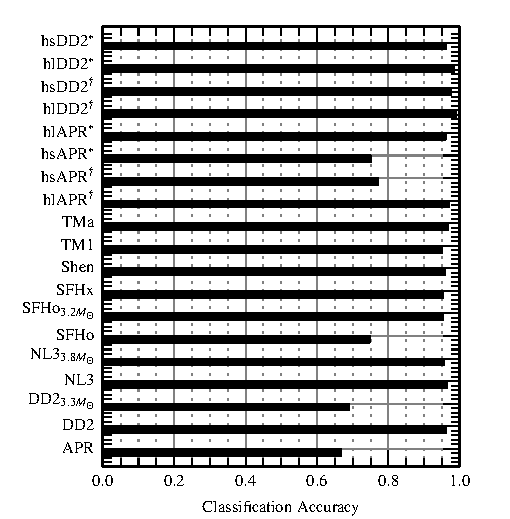
\includegraphics[width=1\columnwidth]{figures/classification.pdf}
                \caption{Probability of identifying correct post-merger scenario}
            \end{figure}
        \end{center}

        \column{0.5\textwidth}

        \begin{center}
            \vspace{-0.5cm}
            \begin{figure}
                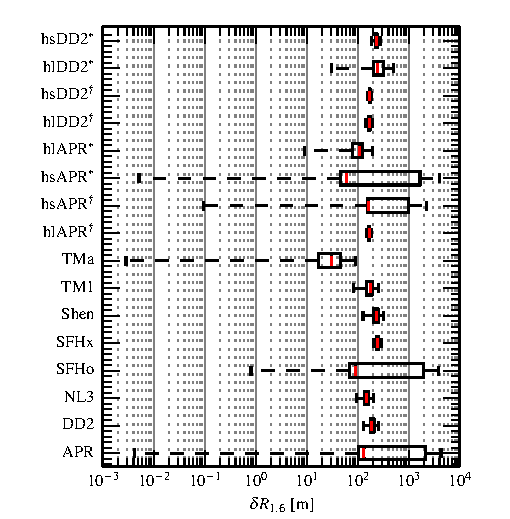
\includegraphics[width=1\columnwidth]{figures/deltaRadii.pdf}
                \caption{Absolute error in radius recovery}
            \end{figure}
        \end{center}

    \end{columns}

\end{frame}


%\begin{frame}
%    \frametitle{Principal Component Analysis Of Short Bursts}
%
%
%
%        \begin{center}
%            \vspace{-0.5cm}
%            \begin{figure}
%                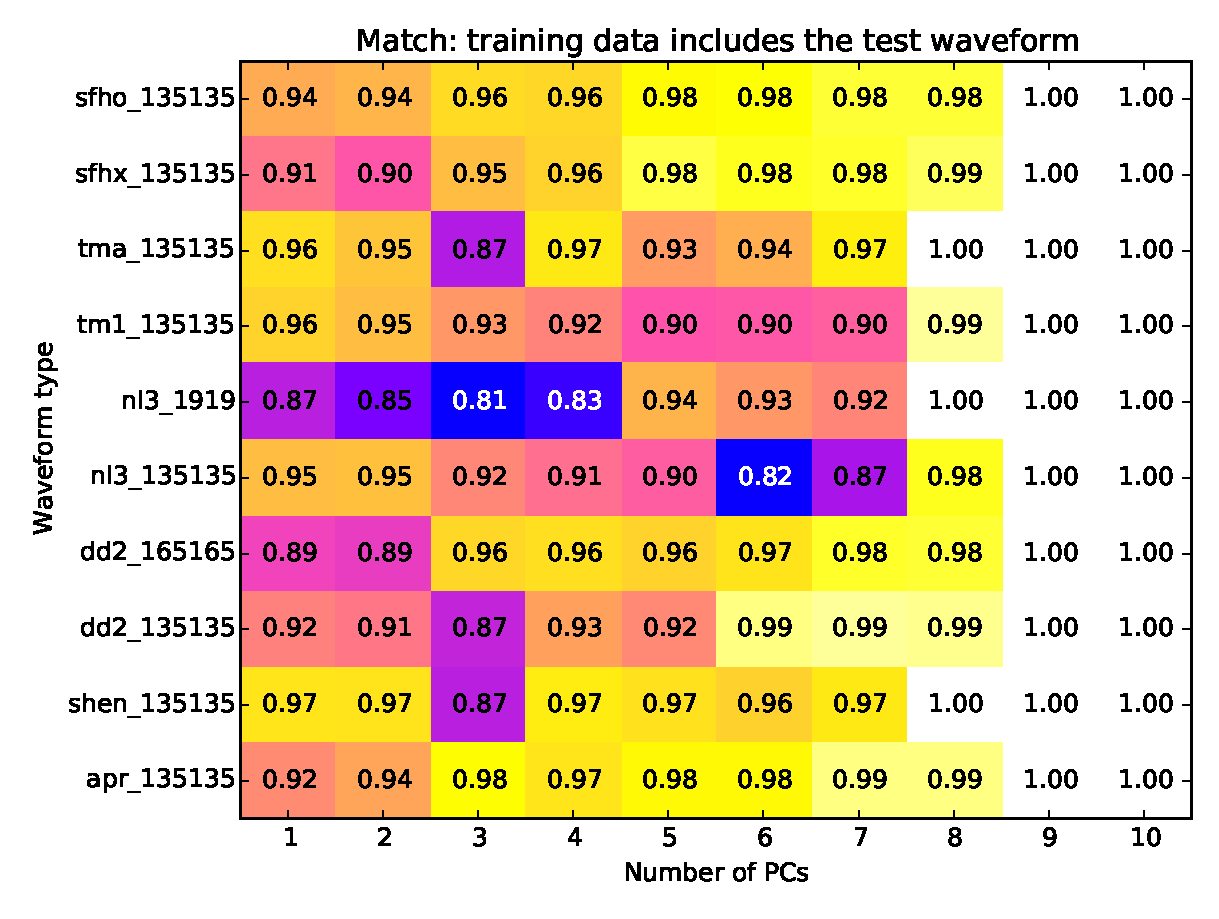
\includegraphics[width=\columnwidth]{figures/match_grid_inctestwav.pdf}
%            \end{figure}
%        \end{center}
%
%\end{frame}
%
%\begin{frame}
%    \frametitle{Principal Component Analysis Of Short Bursts}
%
%        \begin{center}
%            \vspace{-0.5cm}
%            \begin{figure}
%                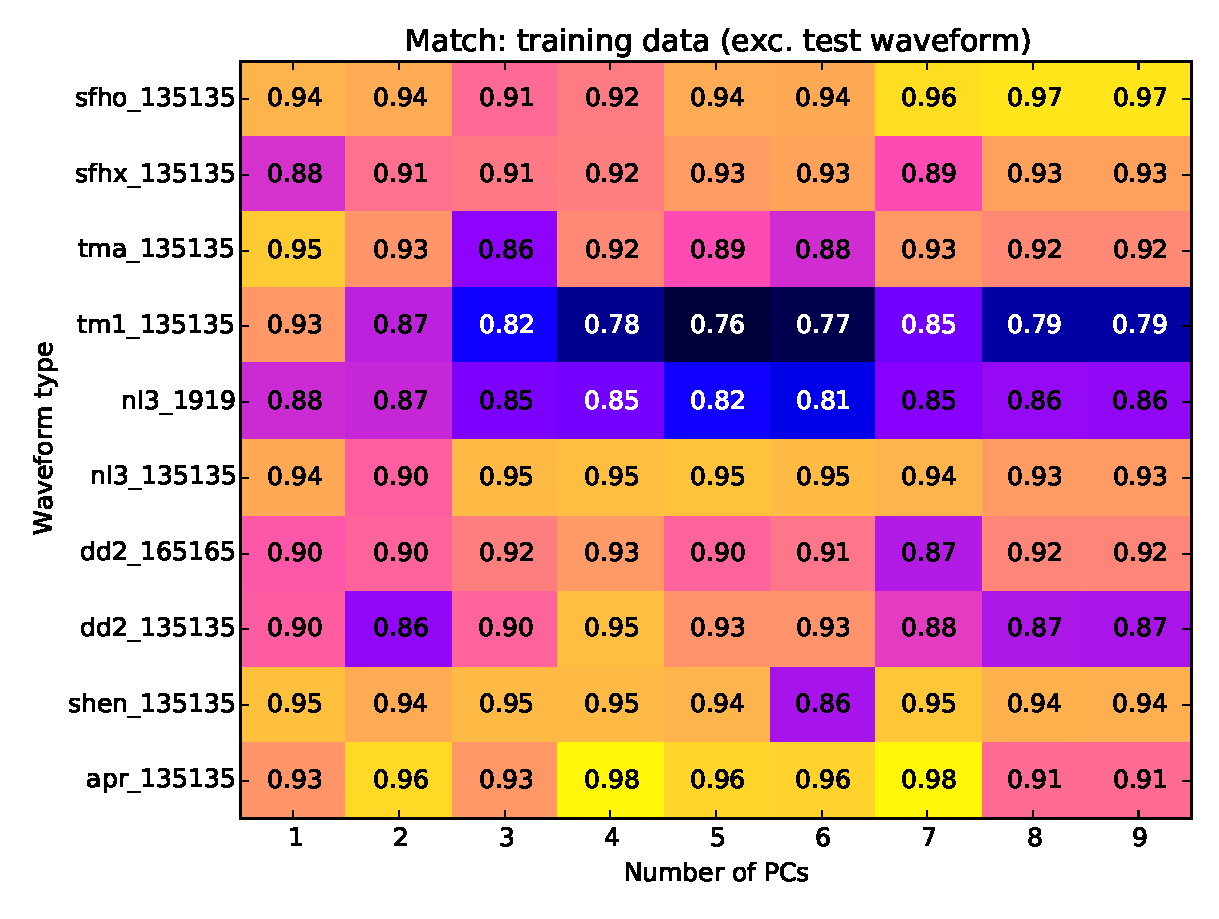
\includegraphics[width=\columnwidth]{figures/match_grid_exctestwav.pdf}
%            \end{figure}
%        \end{center}
%\end{frame}


\end{document}

